\section{Memoria ROM 4x8 \label{sec:s3}}

\begin{center}
	\begin{minipage}{12cm}
		\begin{tcolorbox}[title=Actividad 3]
			 Completar el código de la memoria ROM 4x8 en el lenguaje de su elección. Compilar y simular. Usar el visor RTL para indicar como se implementa después de la síntesis. Implementar en la tarjeta DE2-115.
		\end{tcolorbox}	
	\end{minipage}
\end{center}

La visualización RTL de la memoria ROM 4x8 en Verilog se muestra en la \autoref{fig:ROM4x8_rtl}. Como se observa, la implementación de la memoria ROM de 4 localidades de 8 bits se hace utilizando una instancia de decodificador cuya salida se conecta a un conjunto de compuertas lógicas, demostrando que la implementación de una memoria ROM es similar a la de un decodificador. Las simulaciones para el código en Verilog se visualizan en la \autoref{fig:ROM4x8_WaveBi} en base binaria y en la \autoref{fig:ROM4x8_WaveDe} en base decimal. Se utilizaron todos los valores posibles en la dirección de memoria para observar un comportamiento completo en la salida.

En los Anexos se localiza la descripción de la memoria ROM. Se observa que el código es muy similar al del decodificador visto en la Práctica 1, ya que emplea la estructura \textit{case} dentro de una lista sensible. No obstante, se diferencia en que la ROM puede adquirir el tamaño que sea o hacer uso de cualquier número de localidades, en cambio el decodificador tiene un tamaño estático de $2^{n}$, siendo $n$ el número de bits o tamaño de la variable de control.

\begin{figure}[ht]
	\centering
	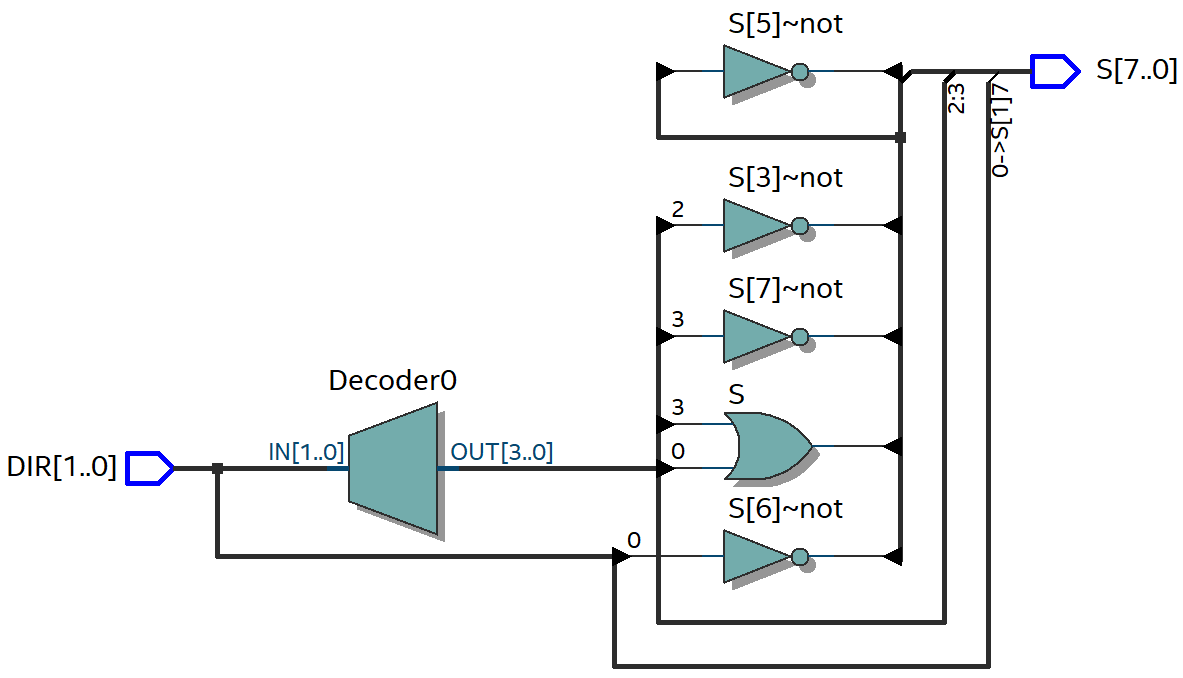
\includegraphics[scale=0.55]{ROM4x8_RTL.png}
	\caption{Diagrama RTL de la memoria ROM 4x8. \label{fig:ROM4x8_rtl}}
\end{figure}

\begin{figure}[ht]
	\centering
	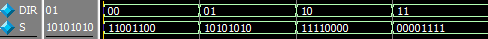
\includegraphics[scale=1.3]{ROM4x8_WaveBi.png}
	\caption{Simulación de la memoria ROM 4x8 con el visor de formas de onda de ModelSim (Base binaria). \label{fig:ROM4x8_WaveBi}}
\end{figure}

\begin{figure}[ht]
	\centering
	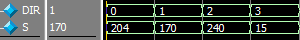
\includegraphics[scale=2]{ROM4x8_WaveDe.png}
	\caption{Simulación de la memoria ROM 4x8 con el visor de formas de onda de ModelSim (Base decimal). \label{fig:ROM4x8_WaveDe}}
\end{figure}